\documentclass[a4paper]{article}

\usepackage[margin=1.5cm]{geometry}  % tweak margins as you like
\usepackage{graphicx}
\usepackage{subcaption}              % only for arranging panels (no sub-captions used)
\pagestyle{empty}
%\usepackage[numbers]{natbib}
%\usepackage[authoryear]{natbib}
\usepackage[numbers]{natbib}
%% The amssymb package provides various useful mathematical symbols
\usepackage{amssymb}
%% The amsmath package provides various useful equation environments.
\usepackage{amsmath}
\usepackage{epstopdf}
\usepackage{mathptmx,mathtools}
\usepackage{subcaption}
\usepackage{float} % Add this in your preamble
\usepackage[export]{adjustbox}
\usepackage{array} % Needed for m{} column type


\usepackage{amsmath}
\usepackage{nicefrac}
\usepackage{dirtytalk}
\usepackage{graphicx}   % For including images
\usepackage{tikz}       % For drawing arrows
\usepackage{xcolor}     % For coloring
\usepackage{lineno}
\renewcommand\linenumberfont{\normalfont\bfseries\small} % <-- Increase line number size

\begin{document}

\setcounter{figure}{1}

\begin{figure}[!tbp]
	\centering
	% First subfigure
	\begin{subfigure}[t]{0.49\textwidth}
		\centering
		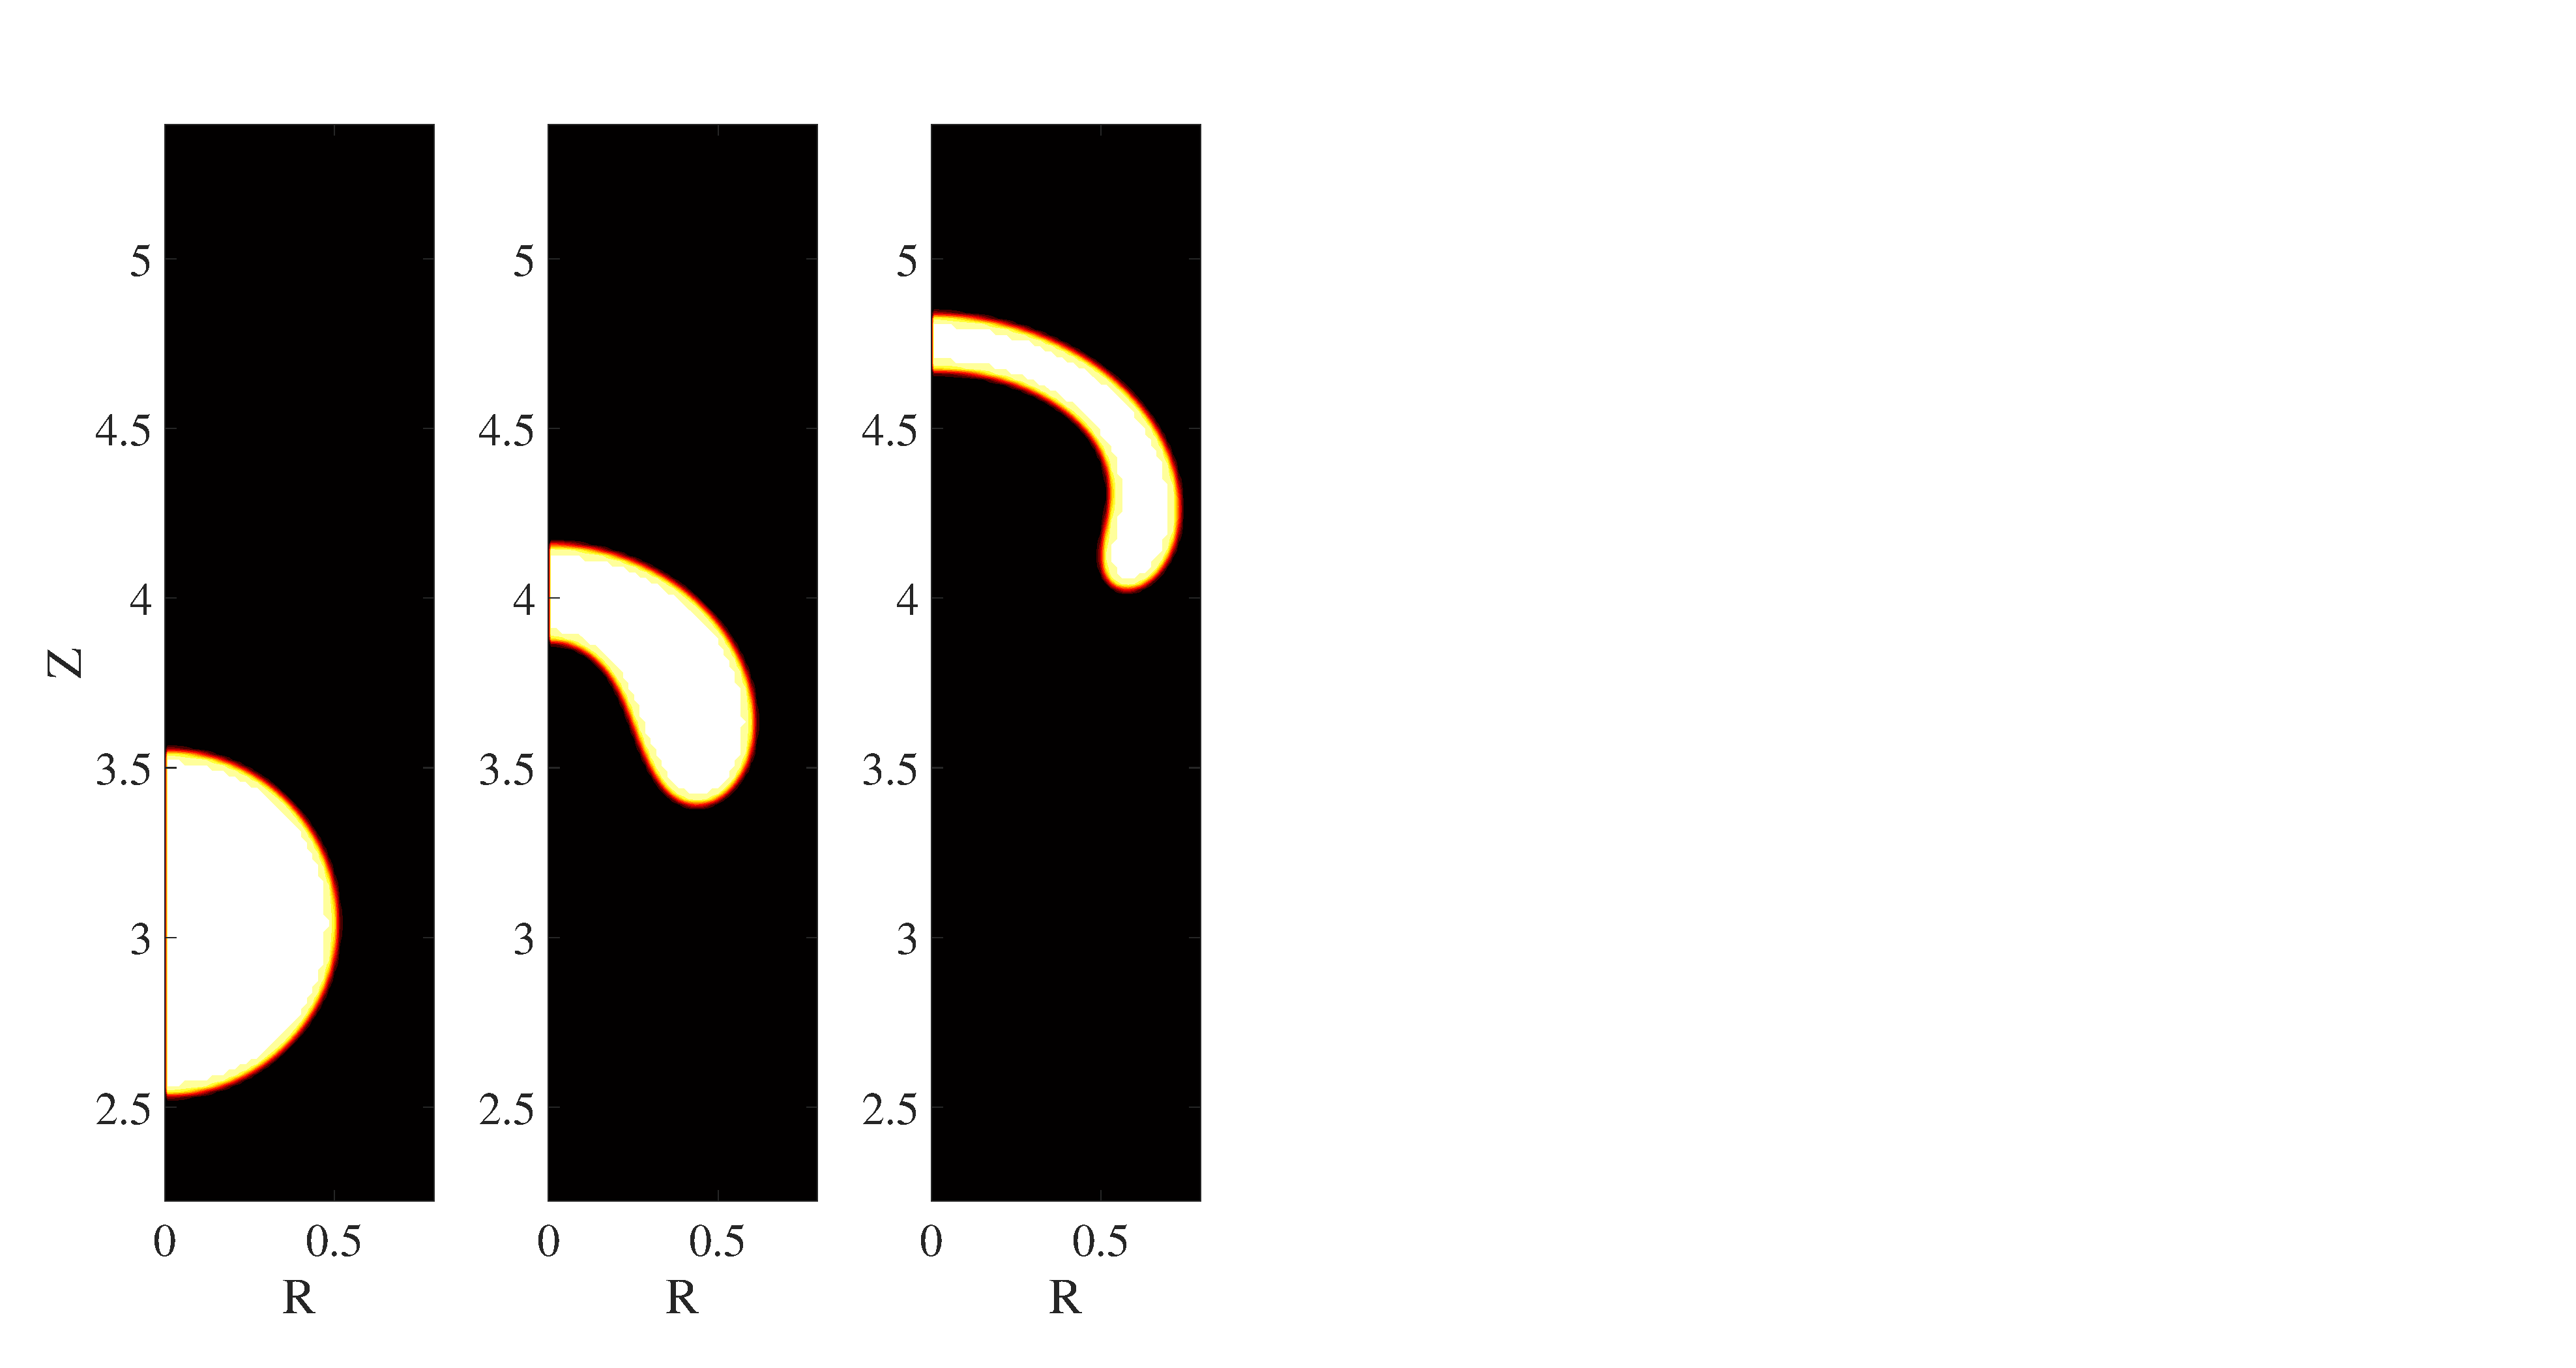
\includegraphics[scale=0.27,trim={0.8cm 1cm 0cm 1cm},clip]{Figure2a.eps}
		\put(-490,250){\large\textbf{(a)}}
	\end{subfigure}
	\hfill
	% Second subfigure
	\begin{subfigure}[t]{0.49\textwidth}
		\centering
		\includegraphics[scale=0.27,trim={0.8cm 1cm 0cm 1cm},clip]{Figure2b.eps}
		\put(-490,250){\large\textbf{(b)}}
		\vspace{0.5cm}
	\end{subfigure}
	% Third subfigure
	\begin{subfigure}[t]{0.49\textwidth}
		\centering
		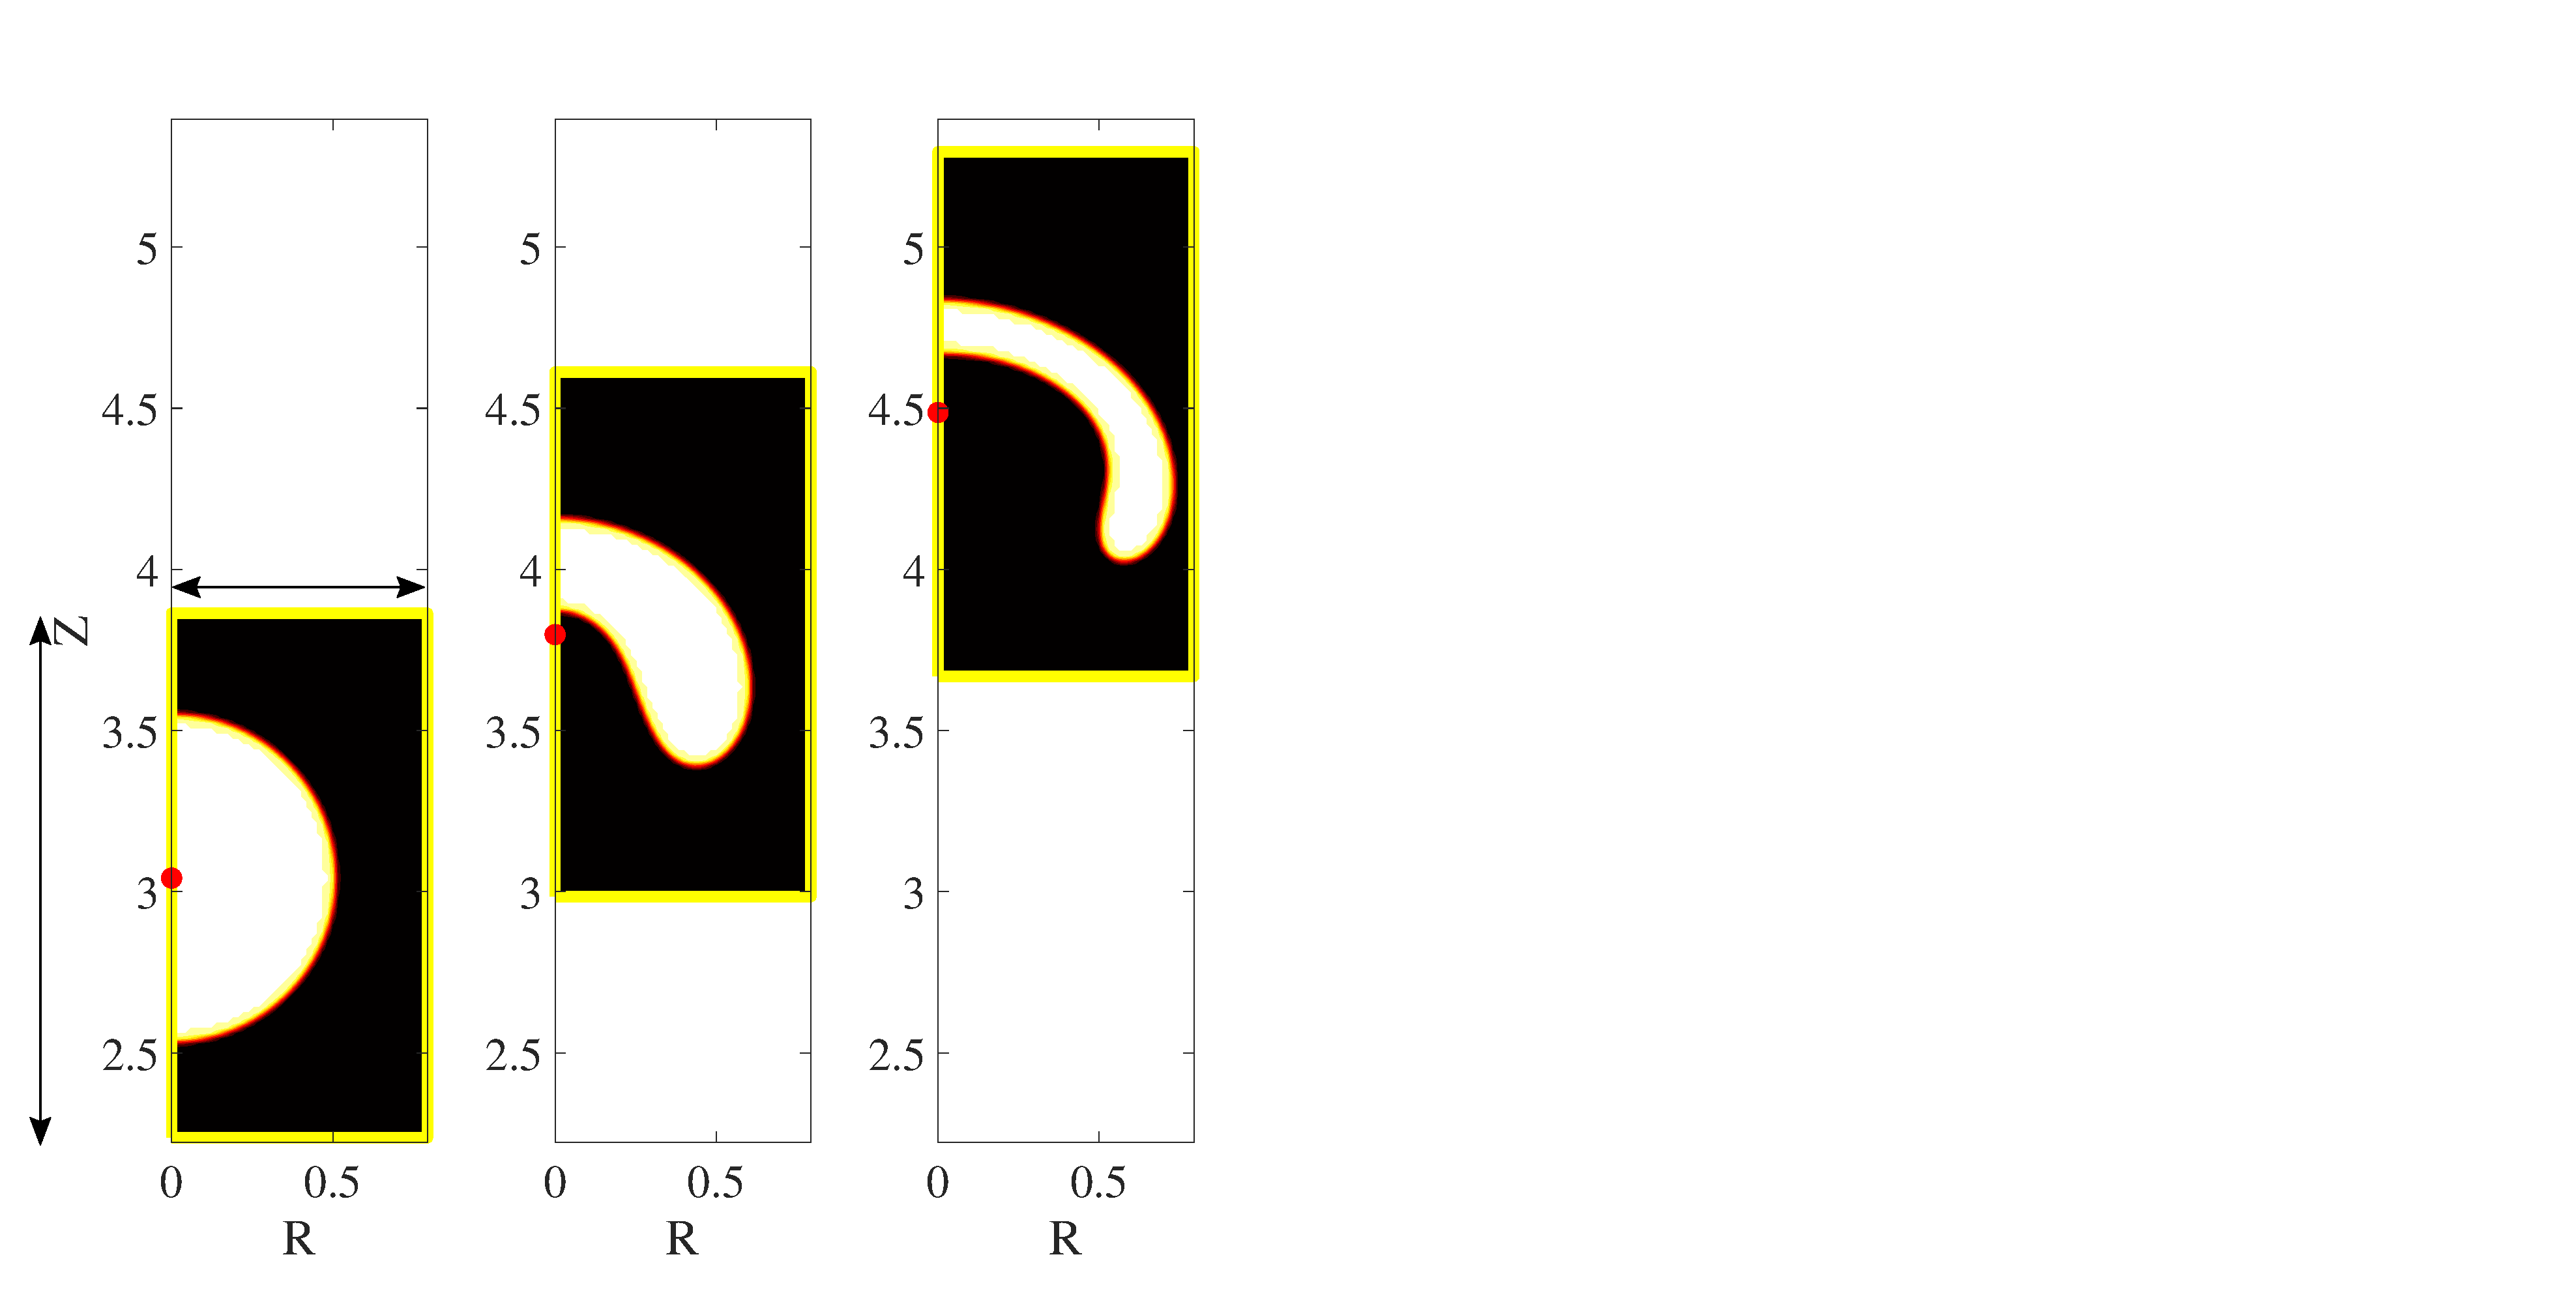
\includegraphics[scale=0.27,trim={0cm 1cm 0cm 1cm},clip]{Figure2c.eps}
		\put(-490,240){\large\textbf{(c)}}
		\put(-468,140){\fontsize{12}{10}\selectfont{0.75D}}
		\put(-535,70){\fontsize{12}{10}\selectfont{1.5D}}
	\end{subfigure}
	\caption{Instantaneous deformation of the rising bubble at three different non-dimensional time~$\tau= 0.10,~4.25,$ and $8$ for the case C$_3$ on a) Eulerian, b) Lagrangian, and c) \textcolor{blue}{Moving-Eulerian} frameworks.}
	\label{Fig2}
\end{figure}

\end{document}